\subsection{Analyzing maximum market potential}
This section presents the results under the scenario with ``ample size" of system to indicate a maximum revenue potential of flexibility solutions in each market regimes. Historical price data is used as fixed input and a generic ESS model without cost elements are adopted. It was found

More details are provide in the reminder of this section.

\subsubsection{Market potential of flexibility solution in PJM}
We first examine the market potential obtained by the scenario with ``ample size" of ESS system, as shown by Figure \ref{fig:germany-ess}. In the figure, we illustrate both the amount of revenue that represents the market potential, and the system size that exhausts the liquidity in the corresponding market to present an intuitive view on the market scale.

\subsubsection{Market potential of flexibility solution in Germany}



\begin{figure}[h!]
	\centering
	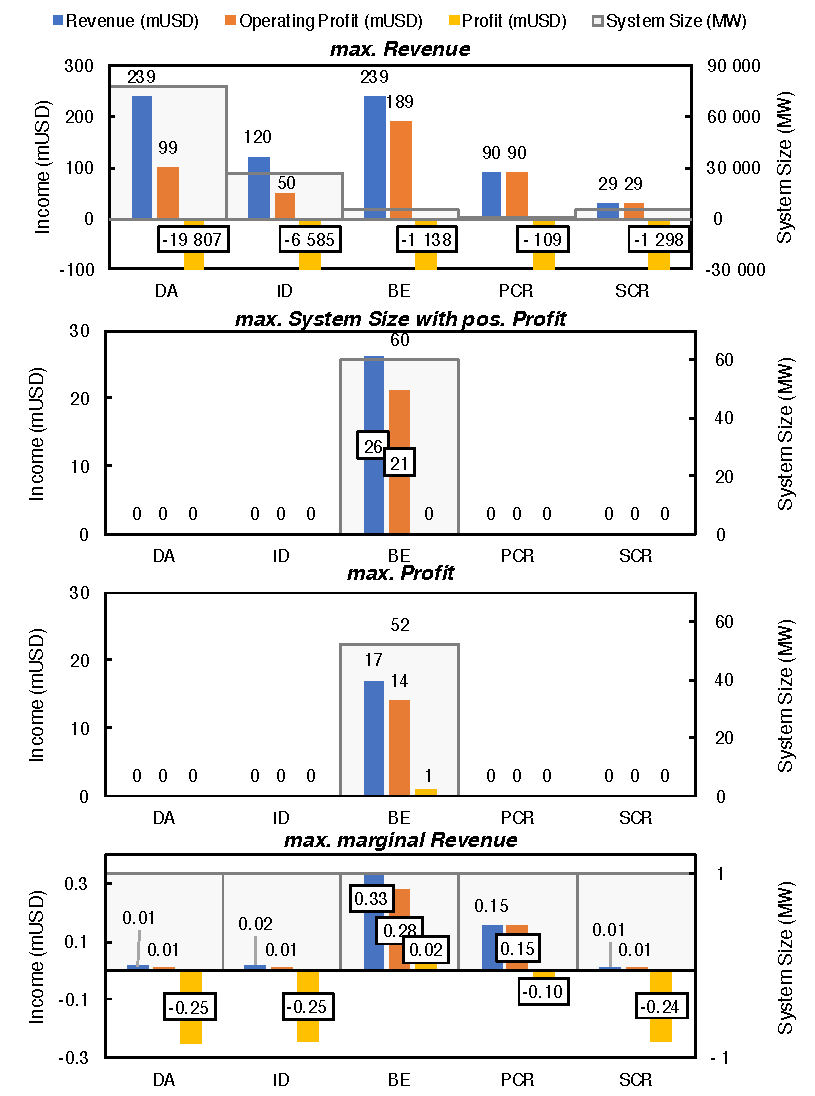
\includegraphics[width=0.9\linewidth]{Figures/Germany_ESS}
	\caption{Market potential of ESS in Germany electricity markets in the scenario with ``ample size" of system}
	\label{fig:germany-ess}
\end{figure}

Overall, the market potentials in different marketplaces are not inspiring for aggregators nor technology vendors. The highest market potential lie in the day-ahead market, which is not surprising since largest proportion of electricity transactions are done through the day-ahead market. However, the revenue potential is merely 4.6 USD/($a\cdot$MP), which is not likely to give end-consumers sufficient incentives to participate, challenging the feasibility of aggregator business. 

However, being corresponded to a total market size of 239 mUSD/$a$ in whole Germany, this business should still be attractive to market players but centralized solutions such as grid-scale battery could be probably more practical options. 

A more interesting finding is seen by comparing the results between self-balancing against balancing energy charges and providing secondary control reserve (SCR): with almost same scale of flexibility system, the revenue from providing self-balancing services for BGs are much higher than providing SCR to TSOs. As we have introduced in Section \ref{sec:quali-de}, the balancing energy price is set to recover part of the cost for procuring SCR and TCR, and to be qualified as SCR providers is more demanding than to be employed by BGs. However, the quantitative results reveals that the latter is actually a more promising use-case for flexibility solutions. 

Comparing the result to the total SCR payments in Germany in 2016 that was 3.4 USD/($a\cdot$MP), only 16.5\% of the market is technically accessible with ESS. Recalling our qualitative analysis that adverse product design especially the non-energy-neutral control signal could be the reason, we adopt the solution proposed in Section \ref{sec:special} to purchase energy from markets to self-neutralize the control signal. The results of such a stacking exercise is depicted by Figure \ref{fig:germany-ess-multitasking}. As we can clearly see, there are indeed perfect synergies between energy market and SCR market. With self-neutralization, 77\% of the SCR market becomes accessible.

\begin{figure}[h!]
	\centering
	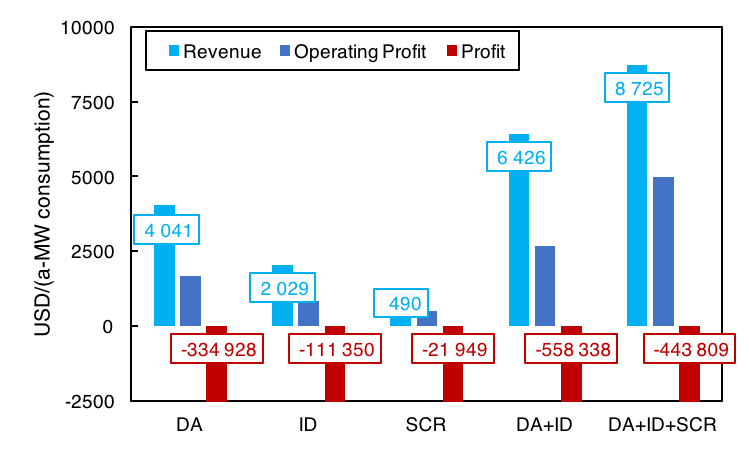
\includegraphics[width=0.95\linewidth]{Figures/Germany_ESS_multitasking}
	\caption{Market potential of ESS with service stacking in Germany electricity markets}
	\label{fig:germany-ess-multitasking}
\end{figure}


\subsection{Valuation of markets under current market conditions}
This section presents the results using historical market data. We first presents the results obtained using technology model of ESS in order to estimate the general market potential for flexibility solutions as well as to evaluate the profitability of BESS. Afterwards, case studies for EV2G are performed.

\subsubsection{ESS in Germany: opportunities hidden by adverse market design of balancing energy and frequency control}


Regarding the profitability using battery, the only profitable use-case is founded to be delivering balancing energy; referring to Figure \ref{fig:germany-ess-profitability}.

\begin{figure}[h!]
	\centering
	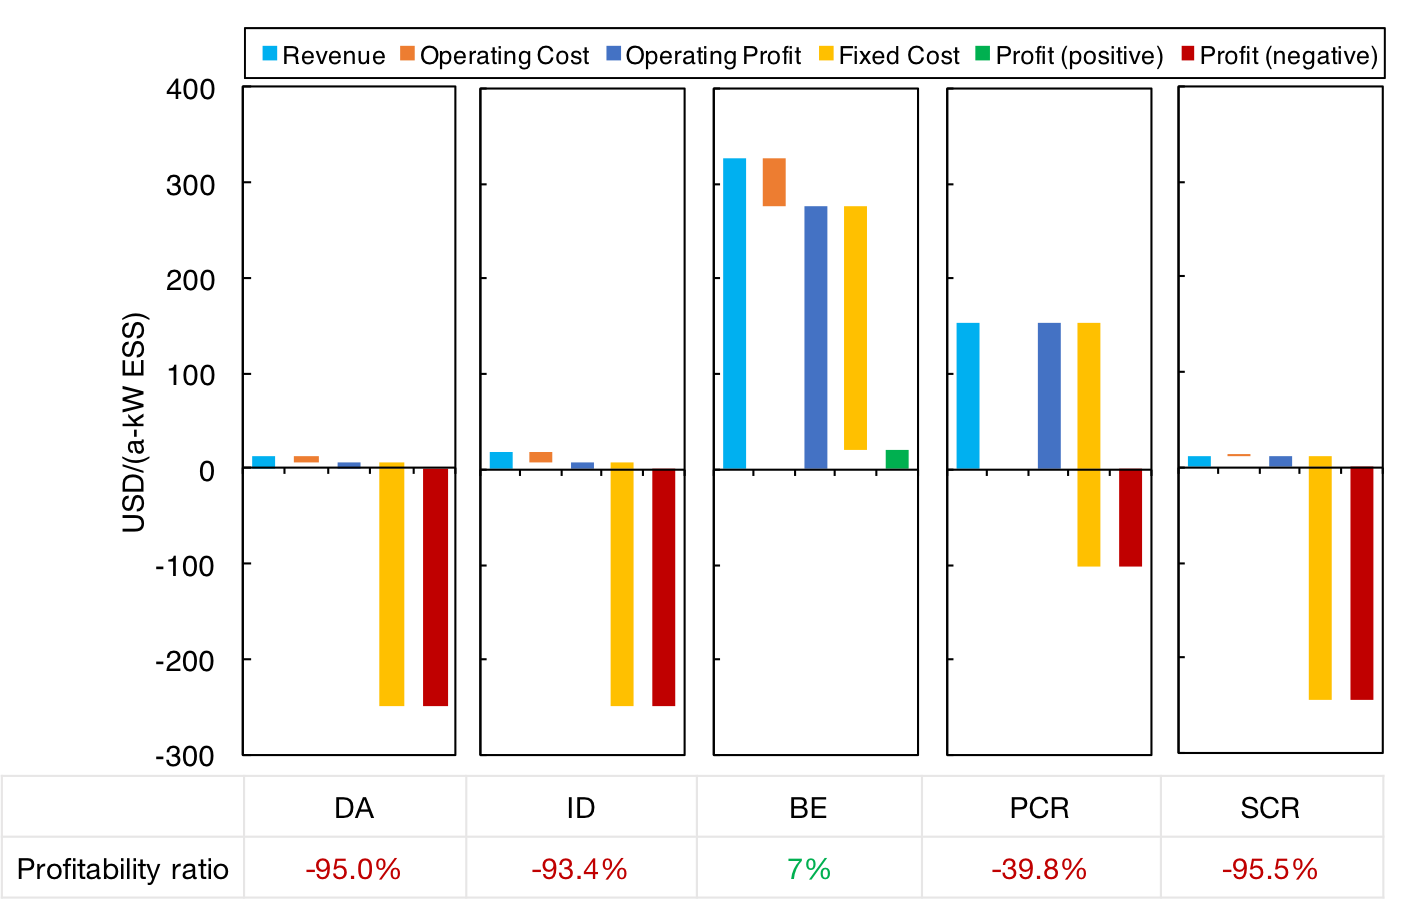
\includegraphics[width=0.9\linewidth]{Figures/Germany_ESS_profitability}
	\caption{Profitability of ESS in Germany electricity markets in the scenario of ``max. marginal Revenue"}
	\label{fig:germany-ess-profitability}
\end{figure}

Together with the indications from market potential analysis, attentions should be indeed raised to
delivering balancing energy services for BGs. 